\begin{frame}{Applying Linear RNNs}
     \vspace{1cm}
     \begin{columns}
     \begin{column}{0.6\textwidth}         
     \begin{itemize}
         \item Speech~\cite{goel2022s}
         \item Video~\cite{Nguyen2022-qi}
         \item RL~\cite{Lu2023-ov}
         \item \textcolor{red}{NLP} 
     \end{itemize}
     \end{column}         
     \begin{column}{0.4\textwidth}         
    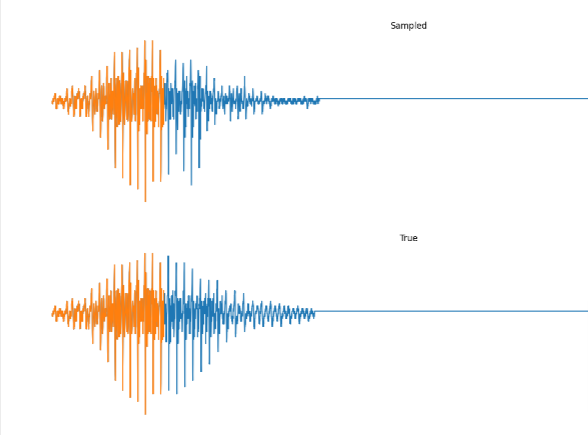
\includegraphics[width=0.9\textwidth, ,clip,trim={0.1cm 0.1cm 0.1cm 0.1cm}]{Figs/speech.png}
     \end{column}         

     \end{columns}    
\end{frame}

\begin{frame}{NLP Results}
    Two types of model
        \vspace{1cm}

    \begin{itemize}
        \item Bidirectional LM (BERT)
        \item Unidirectional LM (GPT)
    \end{itemize}
    \vspace{1cm}
    
    % Different architectures used, Some with partial attention
    
\end{frame}


\begin{frame}{Results: Bidirectional LM \cite{Wang2022-un}}
\begin{figure}
    \centering
    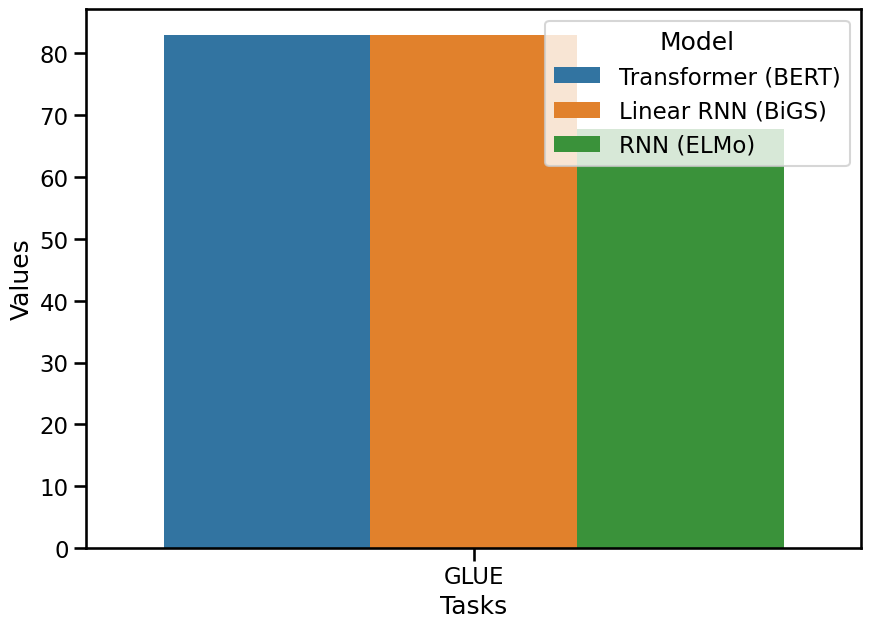
\includegraphics[height=0.6\textheight]{Figs/BiGS.png}
\end{figure}
\end{frame}


\begin{frame}{Analysis: Kernel Visualization $\boldsymbol{\bar{K}}$}

\begin{figure}
    \centering
    \includegraphics[width=\textwidth]{Figs/kernel1.png}
\end{figure}

\begin{itemize}
    \item Replaces Attention Matrix
    \item Single Kernel per layer 
\end{itemize}
\end{frame}

\begin{frame}{Analysis: All Kernels}
\begin{figure}
    \centering
    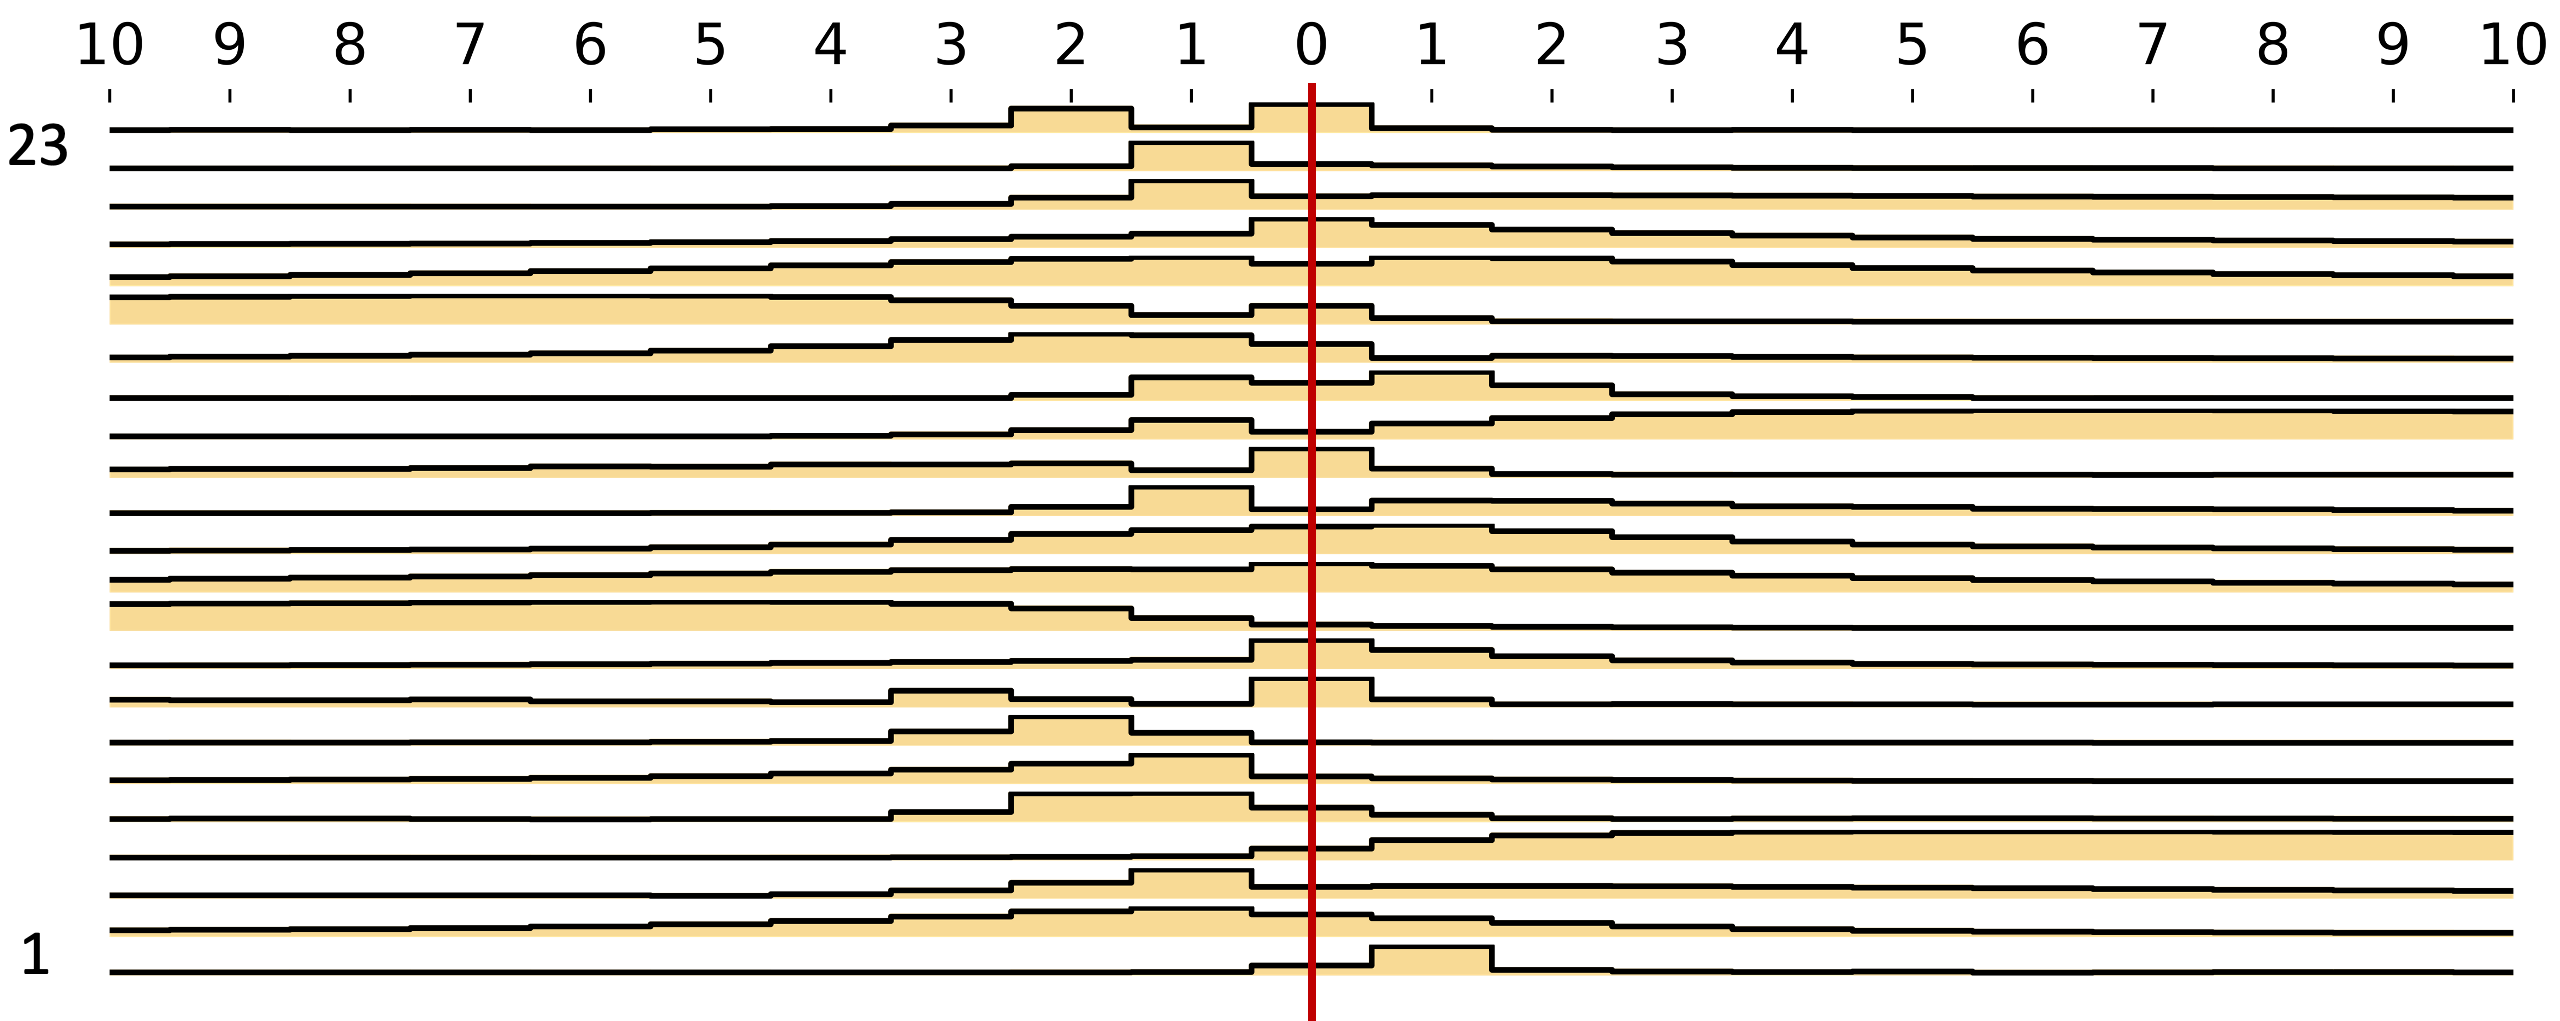
\includegraphics[height=0.6\textheight]{Figs/kernel2.png}
\end{figure}
\end{frame}

\begin{frame}{Analysis: Change in Kernels during Finetuning }

\centerline{Task: Long-Range Sentence Matching}
\begin{figure}
    \centering
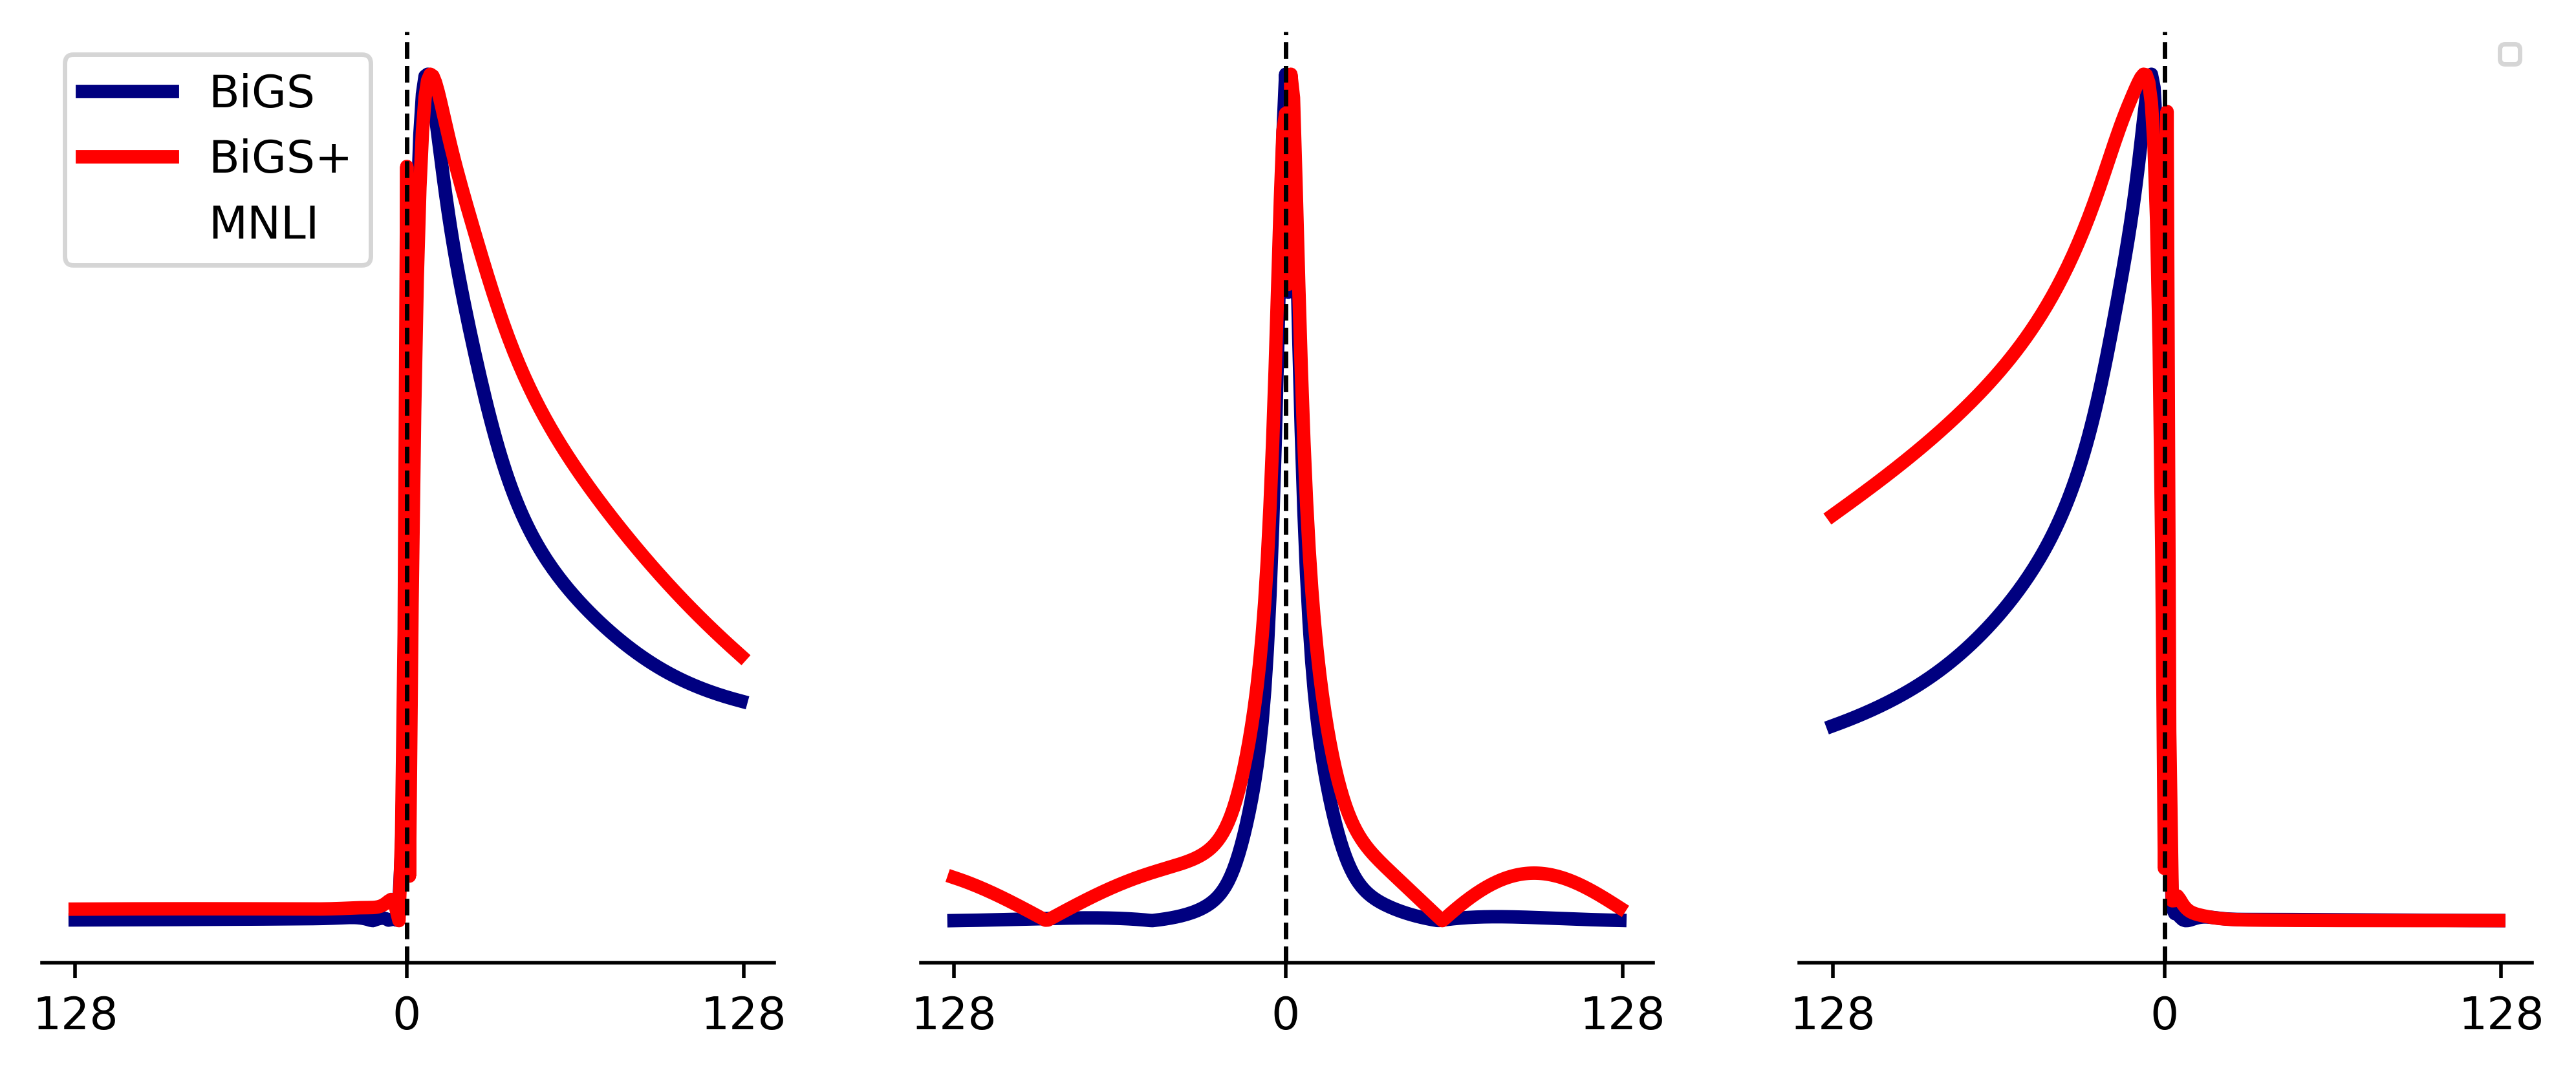
\includegraphics[width=0.8\textwidth]{Figs/comparison_results.png}
    \end{figure}
\end{frame}



\begin{frame}{Results: Unidirectional LM \cite{dao2022hungry}  $\downarrow$}
        \begin{figure}
        \centering
        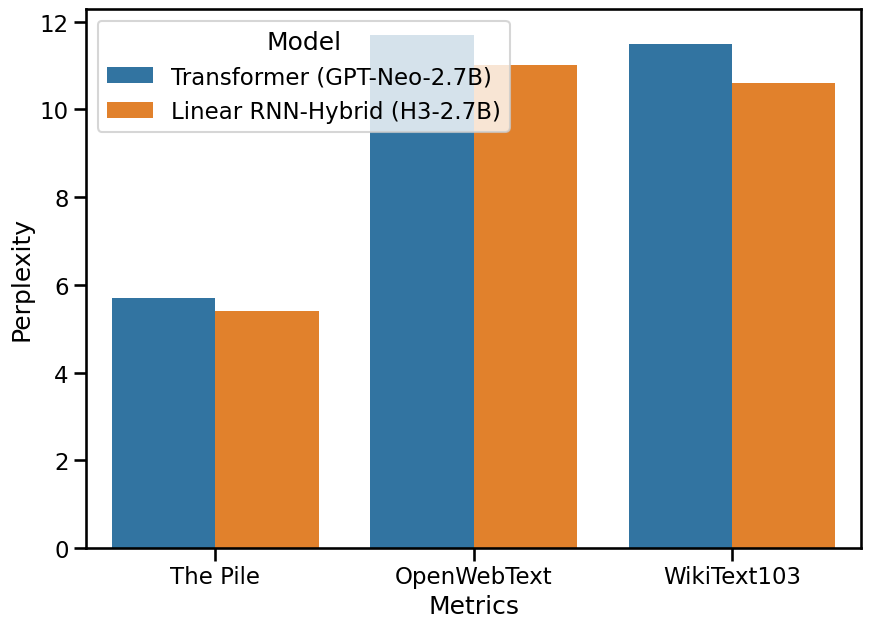
\includegraphics[width=0.7\textwidth]{Figs/H3.png}
        \caption{Caption}
        \label{fig:my_label}
    \end{figure}
\end{frame}

\begin{frame}
    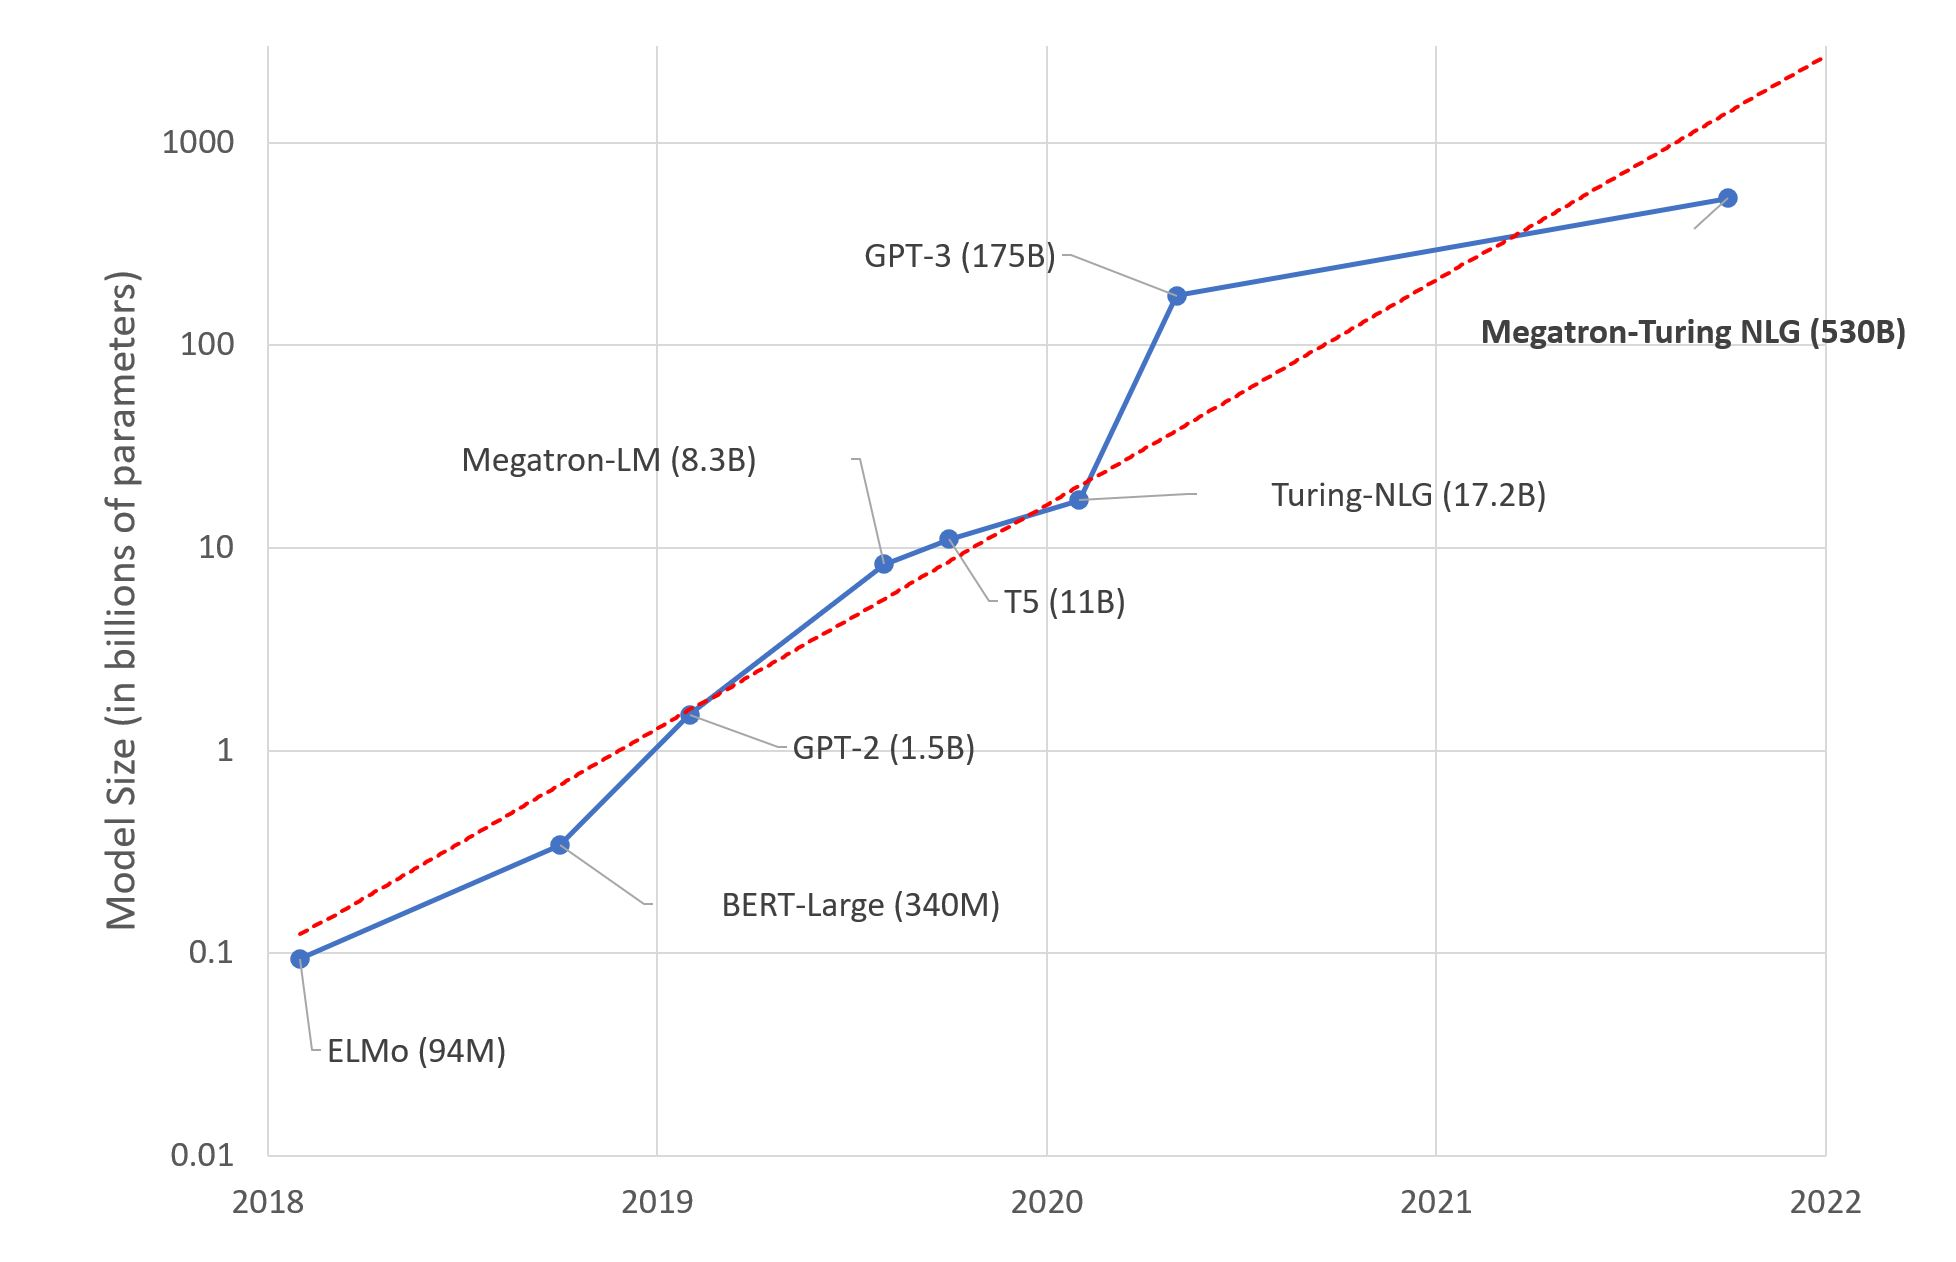
\includegraphics[ clip, height=\textheight]{Figs/ModelSize0.jpg}
\end{frame}

% \begin{frame}{Frame Title}
    
% \end{frame}

\section{Alternative Parameterizations}

\begin{frame}{Do we need the SSM?}
    \begin{figure}
        \centering
            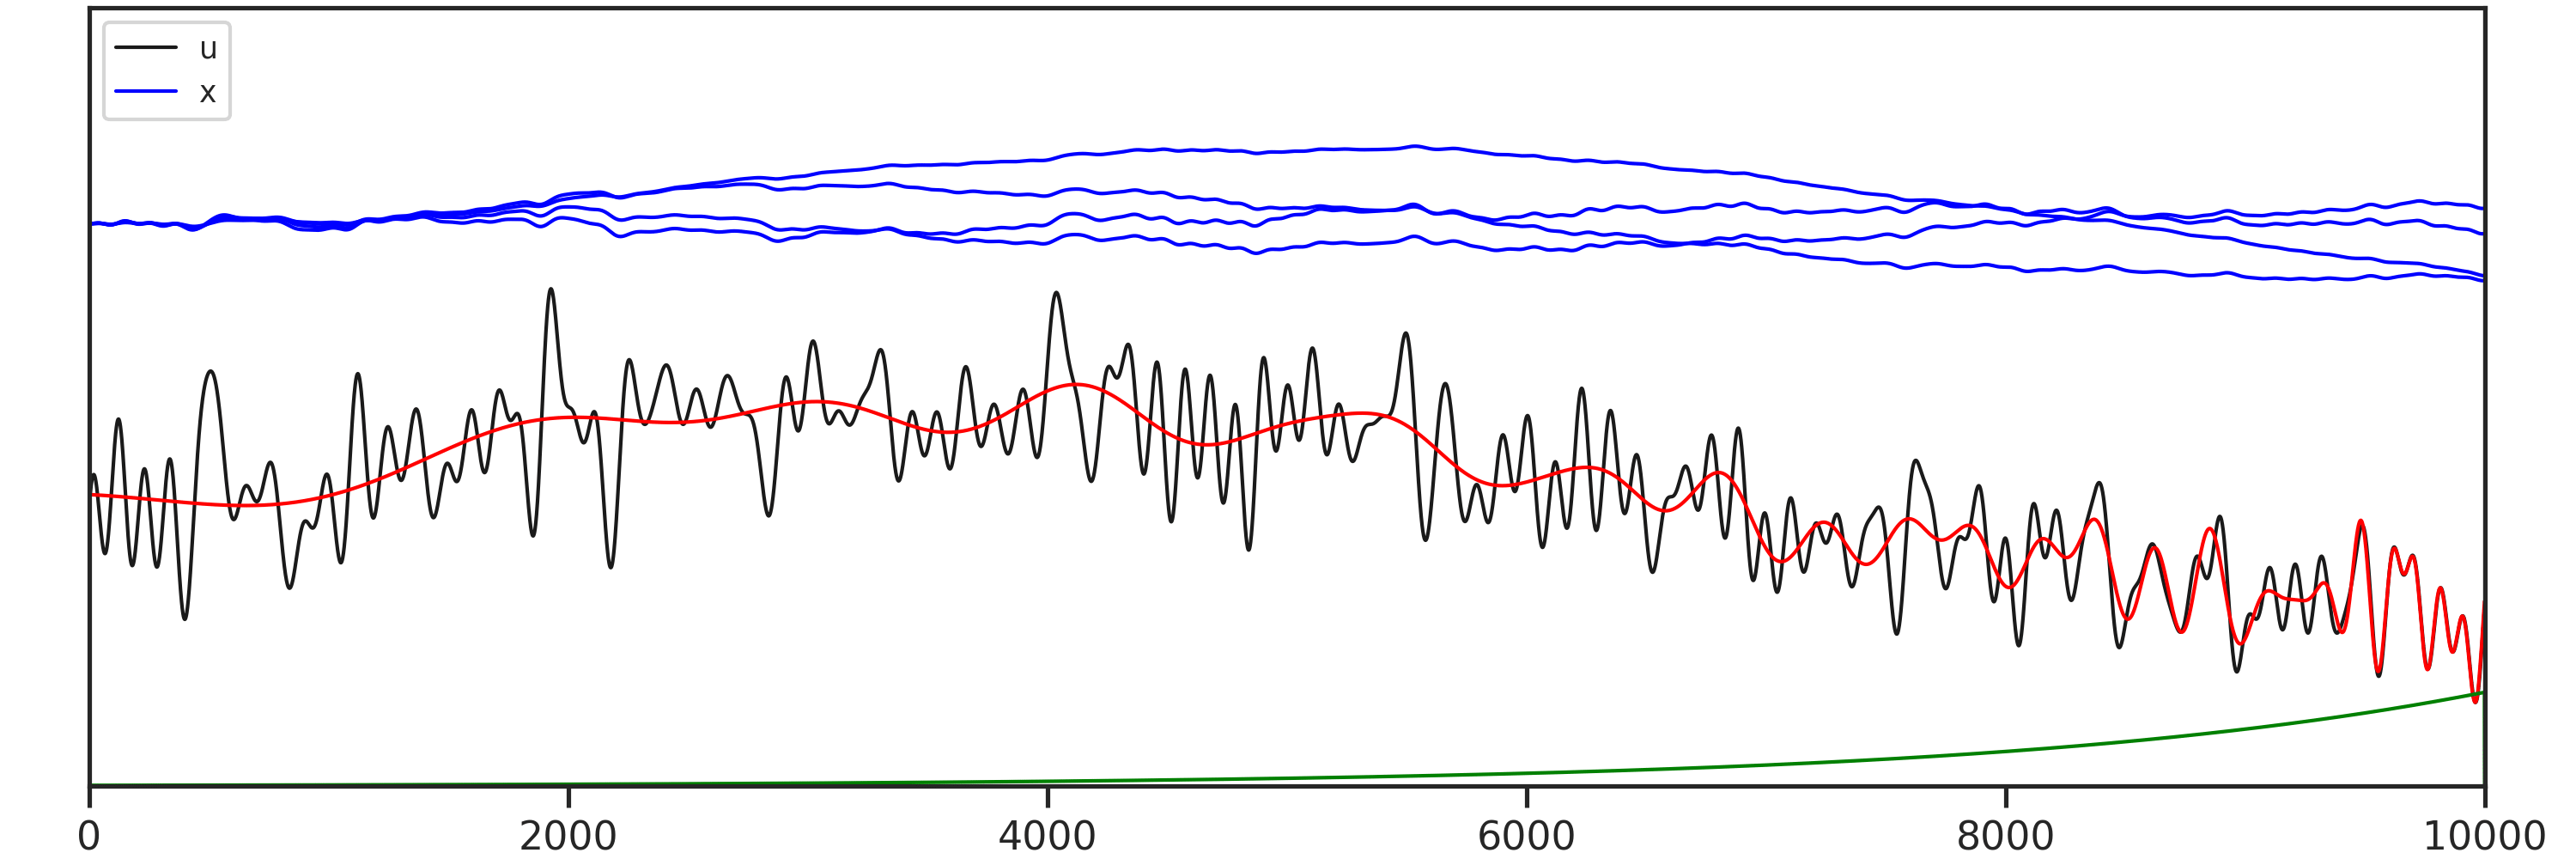
\includegraphics[width=1\textwidth]{Figs/frame_50_delay-0.1s.png}
    \end{figure}
\end{frame}

\begin{frame}{CNN Param: Decaying Structure \cite{Li2022-pn}}
    Parameterization should decay $\bar{K}$ over time.

    \begin{figure}
        \centering
        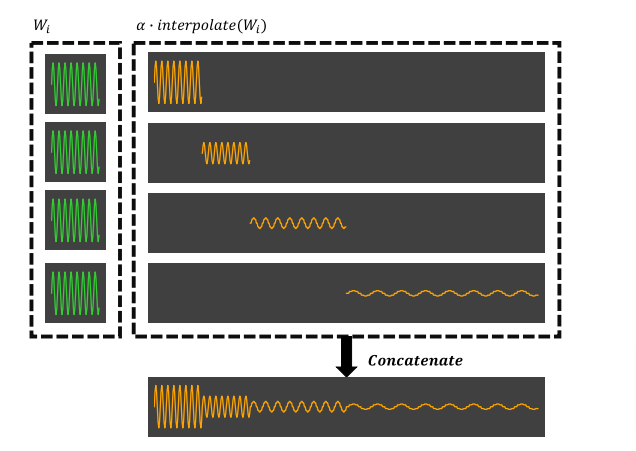
\includegraphics[width=0.4\textwidth]{Figs/sgconv.png}
        \label{fig:my_label}
    \end{figure}

    \begin{figure}
        \centering
        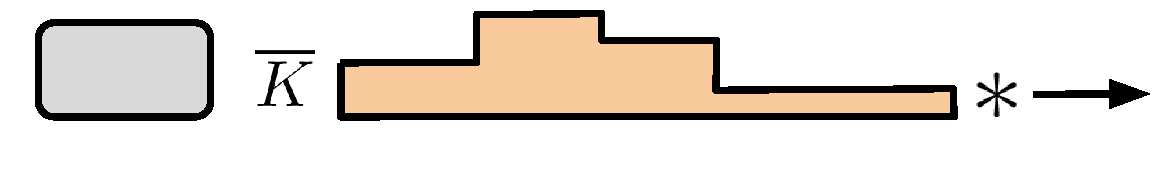
\includegraphics[width=0.5\textwidth]{Figs/SGParam.pdf}
        \label{fig:my_label}
    \end{figure}

\pause
    \begin{center}
    \alert{However}, no linear RNN form.        
    \end{center}
    
\end{frame}



\begin{frame}{RNN Param: LRU \cite{Orvieto2023-an}}
    Stable diagonal parameterization of Linear RNN
    \begin{align*}
    \textcolor{green}{\bar{A}}_{j,j} &= \exp(-\exp({\nu_j}) + i \exp(\theta_j))\\
    \textcolor{blue}{\bar{B}}_{j} &= (1 - |\bar{A}_{j,j}|^2)^{1/2}
    \end{align*}

    \begin{figure}
        \centering
        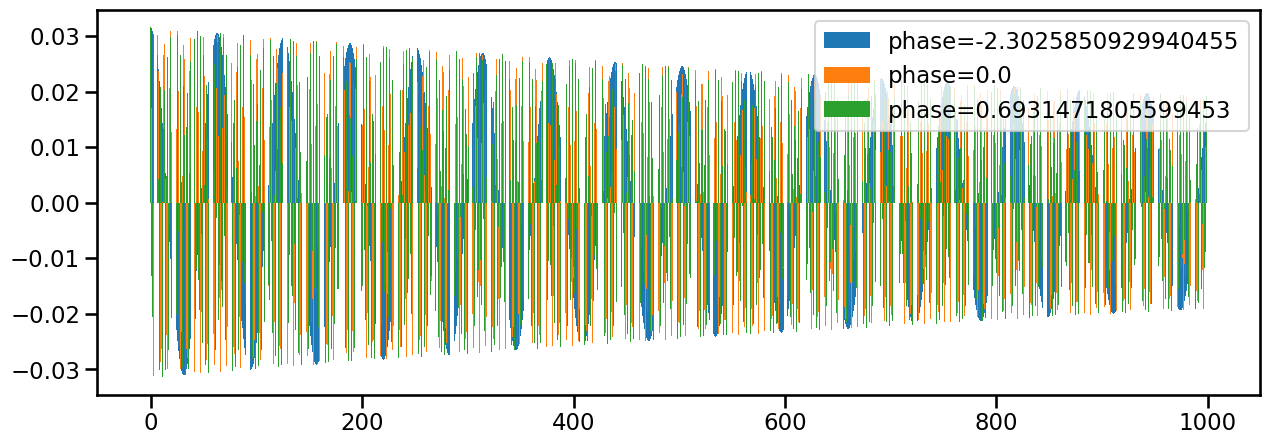
\includegraphics[width=0.8\textwidth]{Figs/phase.png}
        \label{fig:my_label}
    \end{figure}
\end{frame}

\begin{frame}{RNN Param: MEGA \cite{ma2022mega}}
     Use a parameterized damped, exponential moving average
    \begin{align*}
    \textcolor{green}{\bar{A}}_{j,j} &= 1 − \alert{\alpha_j} \times \delta_j \\
    \textcolor{blue}{\bar{B}}_{j} &= \alpha_j
    \end{align*}
    \begin{figure}
        \centering
        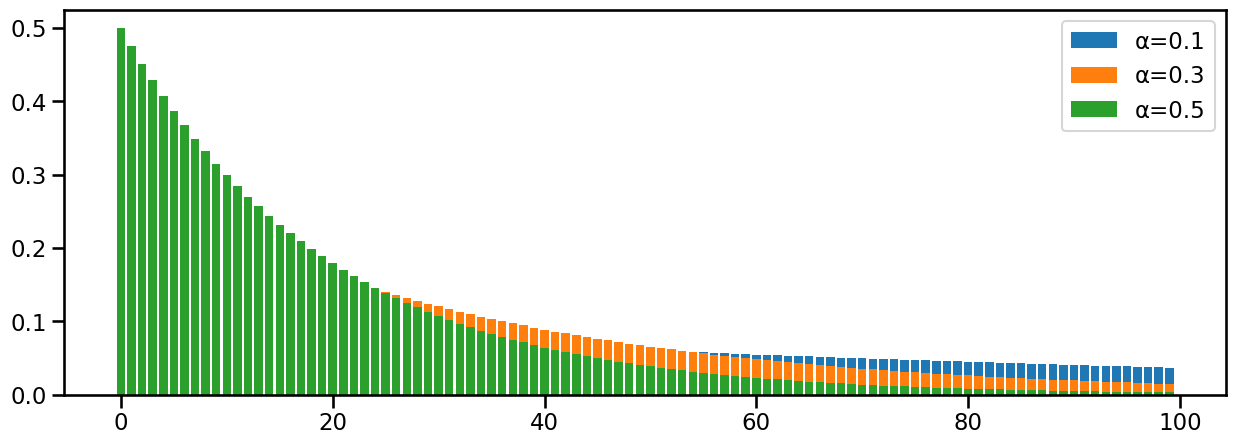
\includegraphics[width=0.7\textwidth]{Figs/ema.png}
        \label{fig:my_label}
    \end{figure}
    \begin{center}
    Very good results on NLP tasks like Translation. 
    \end{center}
    
\end{frame}


\begin{frame}{RNN Param: RWKV \cite{Peng2023-yp}}
    Inspired by Attention 
    
    Split into Keys, Values, and Receptance (no Query):
    \begin{align*}
    K_i, V_i, R_i
    \end{align*}
    \pause 
    Then compute averaged values normalized by keys. 
    
    \begin{align*}
     R_i\frac{\sum_{i'=1}^i \textcolor{green}{\exp(w)}^{i'}\exp(K_{i'}) V_{i'}} {\sum_{i'=1}^i \textcolor{green}{\exp(w)}^{i'}\exp(K_{i'})\phantom{ V_{i'}}} = R_i \frac{\text{LR}_1(\exp(K_i)V_i)}{\text{LR}_2(\exp(K_i))\phantom{V_i}}\\
    \end{align*}

    Yields a product of Linear RNNs (Computed directly).
    
\end{frame}


\begin{frame}{Results: RWKV \cite{Peng2023-yp}}
    \begin{center}
        Largest RNN. Trained up to 14B parameter scale.
    \end{center}
    \pause 
    \begin{figure}
        \centering
        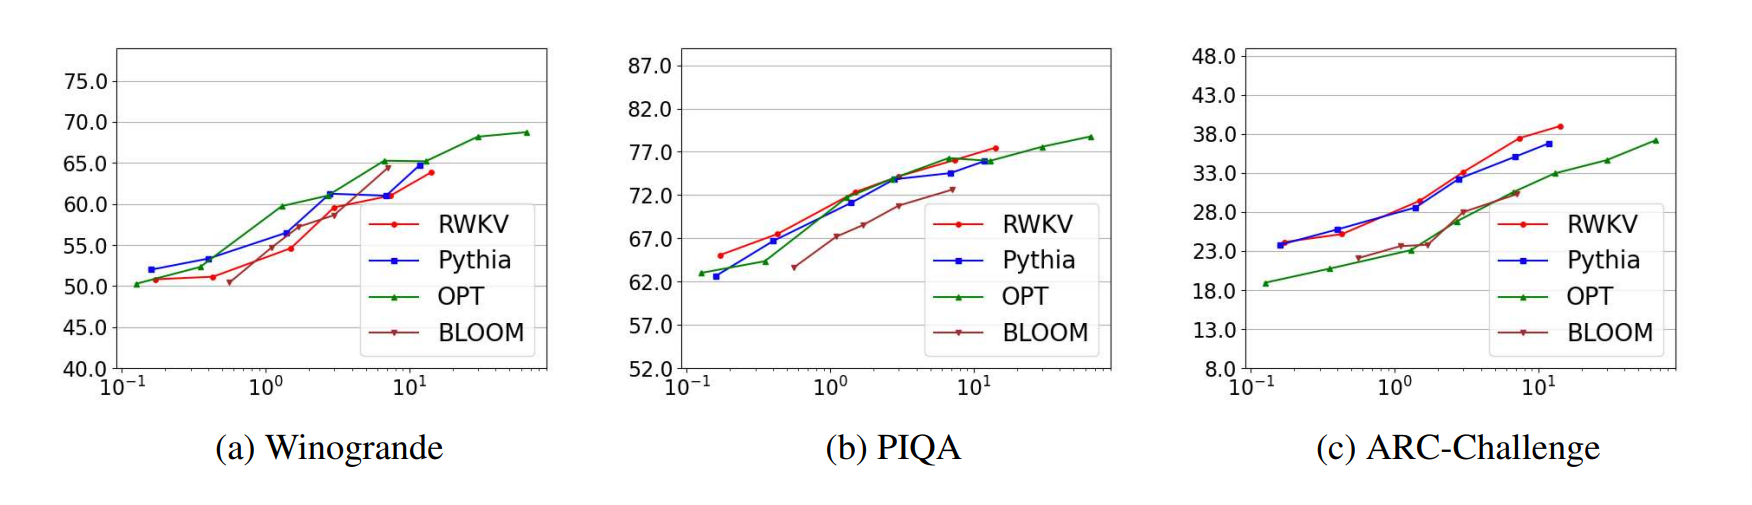
\includegraphics[width=1\textwidth]{Figs/RWKV.png}
        \label{fig:my_label}
    \end{figure}
    Lots of practical interest and community.
\end{frame}


\begin{frame}{Open Question: In-Context Learning}
    \begin{itemize}
        \item Results show comparable loss at medium scales.
        \item Significant interest is in abilities such as in-context learning
        \item Current understanding relies of Attention mechanisms.
    \end{itemize}
\end{frame}


% \begin{frame}{Parameterization: Diagonal RNN \cite{Li2022-pn}}
%     \begin{figure}
%         \centering
%         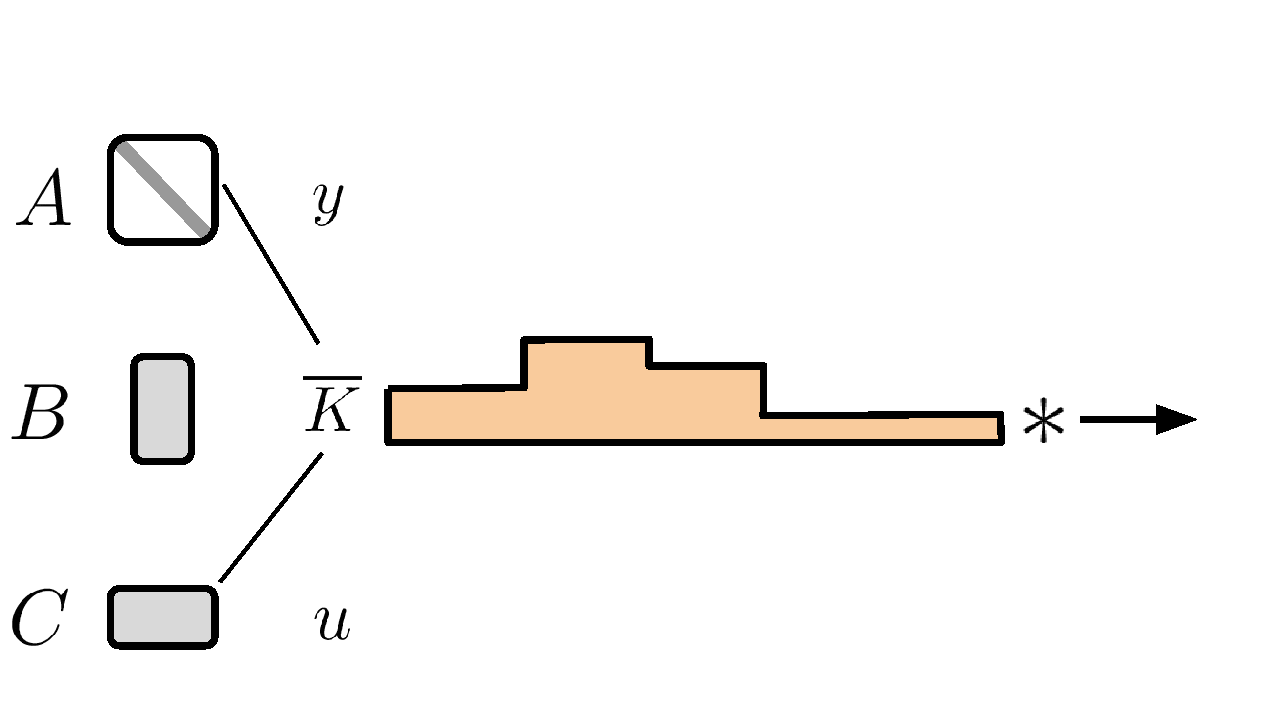
\includegraphics[width=0.5\textwidth]{Figs/DSSM.pdf}

%         \label{fig:my_label}
%     \end{figure}
% \end{frame}

% \begin{frame}{Results: GSS   $\downarrow$}
%         \begin{figure}
%         \centering
%         \includegraphics[width=0.7\textwidth]{}
%         \caption{Caption}
%         \label{fig:my_label}
%     \end{figure}
% \end{frame}





% \begin{frame}{Results: MEGA \cite{ma2022mega} $\uparrow$}
%     \begin{figure}
%         \centering
%         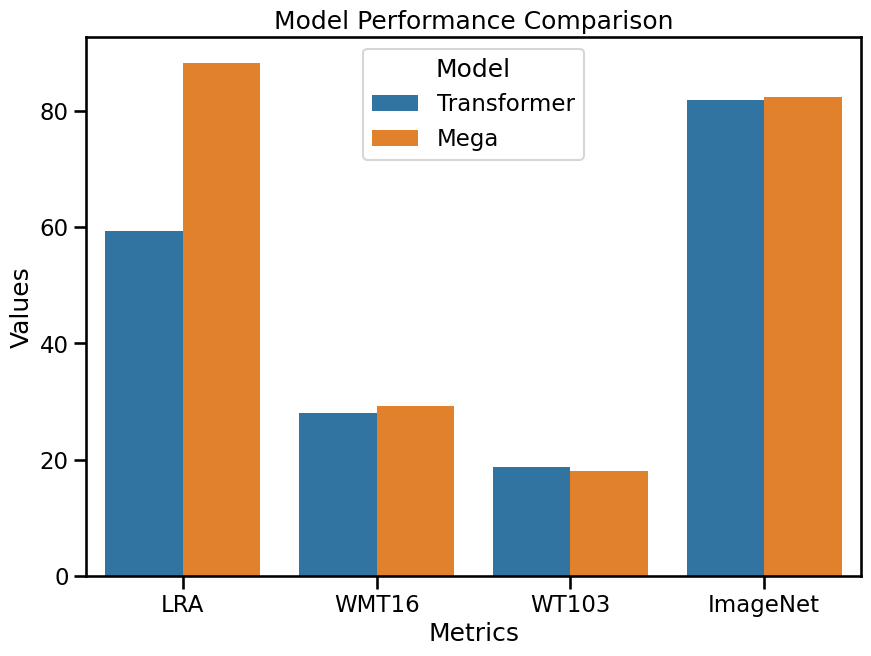
\includegraphics[width=0.7\textwidth]{Figs/Mega.png}
%         \label{fig:my_label}
%     \end{figure}
% \end{frame}
